\documentclass[12pt,titlepage]{article}
\usepackage[margin=1.25in]{geometry}
\usepackage{graphicx,amsmath,enumitem,minted}

%% Variables definition
\newcommand{\vSubject}{Data Structure and Algorithm Practicum}
\newcommand{\vSubtitle}{Final Exam 2nd Semester}
\newcommand{\vName}{Dicha Zelianivan Arkana}
\newcommand{\vNIM}{2241720002}
\newcommand{\vClass}{1i}
\newcommand{\vDepartment}{Information Technology}
\newcommand{\vStudyProgram}{D4 Informatics Engineering}

%% [START] Tikz related stuff
\usepackage{tikz}
\usetikzlibrary{svg.path,calc,shapes.geometric,shapes.misc}
\tikzstyle{terminator} = [rectangle, draw, text centered, rounded corners = 1em, minimum height=2em]
\tikzstyle{preparation} = [chamfered rectangle, chamfered rectangle sep=0.75em, draw, text centered, minimum height = 2em]
\tikzstyle{process} = [rectangle, draw, text centered, minimum height=2em]
\tikzstyle{decision} = [diamond, aspect=2, draw, text centered, minimum height=2em]
\tikzstyle{data}=[trapezium, draw, text centered, trapezium left angle=60, trapezium right angle=120, minimum height=2em]
\tikzstyle{connector} = [line width=0.25mm,->]
%% [END] Tikz related stuff

%% [START] Fancy header related stuff
\usepackage{fancyhdr}
\pagestyle{fancy}
\setlength{\headheight}{15pt} % compensate fancyhdr style
\fancyhead{}
\fancyfoot{}
\fancyfoot[L]{\thepage}
\fancyfoot[R]{\textit{\vSubject - \vSubtitle}}
\renewcommand{\footrulewidth}{0.4pt}% default is 0pt, overline for footer
%% [END] Fancy header related stuff

%% [START] Custom tabular command related stuff
\usepackage{tabularx}
\newcommand{\details}[2]{
    #1 & #2  \\
}
%% [END] Custom tabular command related stuff

%% [START] Figure related stuff
\newcommand{\image}[3][1]{
    \begin{figure}[h]
        \centering
        \includegraphics[#1]{#2}
        \caption{#3}
        \label{#3}
    \end{figure}
}
%% [END] Figure related stuff

\begin{document}
\begin{titlepage}
    \centering
    \vfill
    {\bfseries\LARGE
        \vSubject\\
        \vskip0.25cm
        \vSubtitle
    }
    \vfill
    
\includegraphics[width=6cm]{images/polinema-logo.png}
    \vfill
    {
        \textbf{Name}\\
        \vName\\
        \vskip0.5cm
        \textbf{NIM}\\
        \vNIM\\
        \vskip0.5cm
        \textbf{Class}\\
        \vClass\\
        \vskip0.5cm
        \textbf{Department}\\
        \vDepartment\\
        \vskip0.5cm
        \textbf{Study Program}\\
        \vStudyProgram
    }
\end{titlepage}

\section{Questions}
\begin{enumerate}[label=\alph*)]
    \item {
        \texttt{toArray():} method in akan menghasilkan sebuah variable array,\\
        dimana datanya berasal dari data di dalam objek linked list yang sudah ada.

        \begin{minted}[autogobble,fontsize=\footnotesize]{java}
            int[] toArray() {
                // prepare the array
                int[] result = new int[this.size()];

                // iterate through the linked list
                Node2P tmp = head;
                for (int i = 0; i < result.length; i++) {
                    // place each of the node inside the array and then advance to the next node
                    result[i] = tmp.data;
                    tmp = tmp.next;
                }

                // return the filled array
                return result;
            }
        \end{minted}
    }
    \item {
        \texttt{sublist(int start, int end):} method ini digunakan untuk mengembalikan list baru
        yang mengambil sebagian dari data yang sudah ada di list dari posisi \texttt{start} sampai posisi \texttt{end}

        \begin{minted}[autogobble,fontsize=\footnotesize]{java}
            DLL sublist(int start, int end) {
                // prepare the linked sub-list container
                DLL subLinkedList = new DLL();

                // keep track of the current index
                int i = 0;
                // walk through the linked list
                Node2P tmp = head;
                while (tmp != null) {
                    // after reaching certain index, add them to the sub-list
                    // we don't use the existing `get(int index)` method since it will
                    // always iterate from the start everytime we want to get an item
                    // (which would make the time complexity to be O(n^2)) while using this
                    // method we'll only have to do a single pass (which will make it O(n))
                    // since the list is within a range
                    if (i >= start && i <= end) {
                        subLinkedList.addLast(tmp.data);
                    }
                    // increment the counter and advance to the next node
                    i++;
                    tmp = tmp.next;
                }

                // return the filled sub linked list
                return subLinkedList;
            }
        \end{minted}
    }
    \item {
        \texttt{addAll(DLL list):} method ini digunakan untuk menambahkan data yang ada di \texttt{list} ke dalam list yang sudah ada

        \begin{minted}[autogobble,fontsize=\footnotesize]{java}
            void addAll(DLL list) {
                // iterate through every node in the list in the parameter and
                // then add it to the list of this class
                Node2P tmp = list.head;
                while (tmp != null) {
                    // add each item from the passed list to the last of the existing list
                    this.addLast(tmp.data);
                    tmp = tmp.next;
                }
            }
        \end{minted}
    }
    \item {
        \texttt{containsAll(Dll list):} method ini akan mengecek apakah semua data yang ada di dalam \texttt{list}, ada di dalam list yang sudah ada

        \begin{minted}[autogobble,fontsize=\footnotesize]{java}
            boolean containsAll(DLL list) {
                // walk through every nodes
                Node2P tmp = list.head;
                while (tmp != null) {
                    // create a flag that marks if the item of the list contained in the class' list
                    boolean contains = false;

                    // walk through the list passed from the parameter
                    Node2P innerTmp = head;
                    while (innerTmp != null) {
                        // check if the data is the same in the list, if it does then 
                        // mark the flag as true
                        if (innerTmp.data == tmp.data) {
                            contains = true;
                        }
                        innerTmp = innerTmp.next;
                    }

                    // if at the end of the loop the flag remains false, it means that
                    // there is no item from the passed list in the class' list, so we'll
                    // just return false here and stop the loop, no need to check the rest
                    if (!contains) return false;
                    tmp = tmp.next;
                }

                // returns true when the above loop passes
                return true;
            }
        \end{minted}
    }
    \pagebreak
    \item {
        \texttt{removeAll(DLL list):} method ini akan menghapus data dari dalam list yang sudah ada berdasarkan nilai yang ada di dalam \texttt{list}

        \begin{minted}[autogobble,fontsize=\footnotesize]{java}
           void removeAll(DLL list) {
                // iterate through the passed list
                Node2P tmp = list.head;
                while (tmp != null) {
                    // remove the item from the list
                    // this would imply O(n^2) since we need to iterate through the inner list
                    // to find the data that we want to delete based on the list that is passed
                    this.deleteByData(tmp.data);
                    tmp = tmp.next;
                }
            }
        \end{minted}
    }
\end{enumerate}

\pagebreak

\section{Output}
\begin{figure}[h]
    \centering
    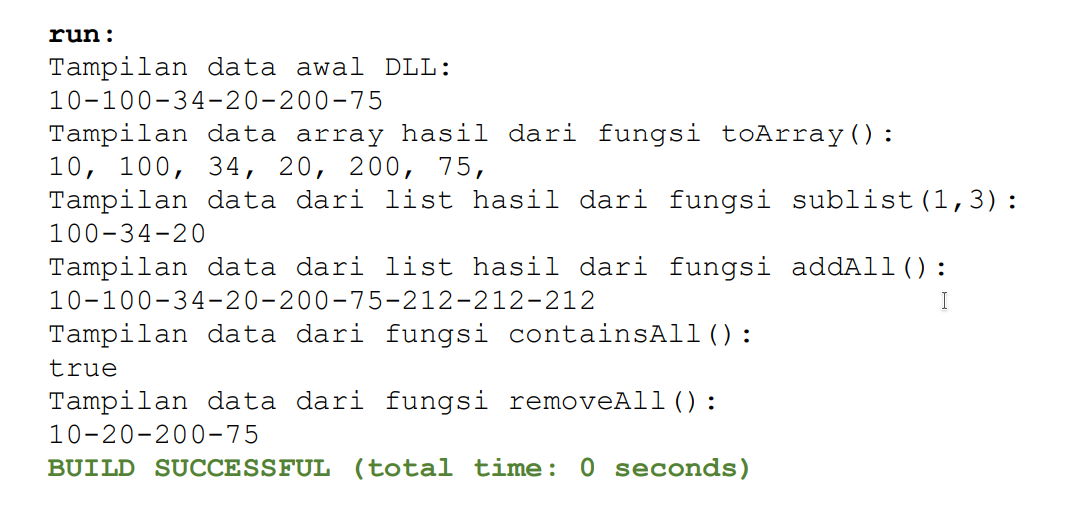
\includegraphics[width=.8\textwidth]{./images/output-reference.png}
    \caption{The expected output of the program}
\end{figure}

\begin{figure}[h]
    \centering
    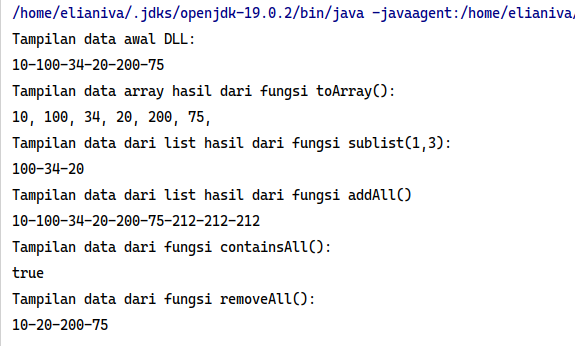
\includegraphics[width=.8\textwidth]{./images/output.png}
    \caption{The actual output of the program}
\end{figure}


\end{document}

